\documentclass[10pt, oneside]{article}
\usepackage[a4paper, total={5.5in, 9in}]{geometry}
\usepackage[ngerman]{babel}
\usepackage{import}

\import{../../.texit/include/}{preamble}

\title{Technische Informatik\\[10pt]\Large{WiSe 2024/25}\\[15pt]\Large{{\"U}bungsblatt 2}}
\author{Volodymyr But\\[10pt]Hochschule Trier}
\date{}

% - - - - - - - - - - - - - - - - - - - - - - - - - - - - - - - - - - - - - - %

\begin{document}
\sloppy

\maketitle
\vspace{25px}

\section{Aufgabe 1}

In der Wertetabelle fehlen die Werte f"ur das Segment d. Erg"anzen Sie diese.
Welche Segmente m"ussen \enquote{on} sein um das Zeichen f"ur 5 darzustellen?

\vspace{5pt}

\begin{minipage}{0.69\linewidth}
    \bgroup
    \def\arraystretch{1.25}
    \begin{tabular}{|c|c|c|c|c|c|c|c|c|c|c|c|}
        \hline
        $x_3$ & $x_2$ & $x_1$ & $x_0$ & Zeichen & $a$        & $b$        & $c$        & $d$               & $e$        & $f$        & $g$        \\
        \hline
        0     & 0     & 0     & 0     & 0       & 1          & 1          & 1          & \textbf{1}        & 1          & 1          & 0          \\
        \hline
        0     & 0     & 0     & 1     & 1       & 0          & 1          & 1          & \textbf{0}        & 0          & 0          & 0          \\
        \hline
        0     & 0     & 1     & 0     & 2       & 1          & 1          & 0          & \textbf{1}        & 1          & 0          & 1          \\
        \hline
        0     & 0     & 1     & 1     & 3       & 1          & 1          & 1          & \textbf{1}        & 0          & 0          & 1          \\
        \hline
        0     & 1     & 0     & 0     & 4       & 0          & 1          & 1          & \textbf{0}        & 0          & 1          & 1          \\
        \hline
        0     & 1     & 0     & 1     & 5       & \textbf{1} & \textbf{0} & \textbf{1} & \textbf{1}        & \textbf{0} & \textbf{1} & \textbf{1} \\
        \hline
        0     & 1     & 1     & 0     & 6       & 1          & 0          & 1          & \textbf{1}        & 1          & 1          & 1          \\
        \hline
        0     & 1     & 1     & 1     & 7       & 1          & 1          & 1          & \textbf{0}        & 0          & 0          & 0          \\
        \hline
        1     & 0     & 0     & 0     & 8       & 1          & 1          & 1          & \textbf{1}        & 1          & 1          & 1          \\
        \hline
        1     & 0     & 0     & 1     & 9       & 1          & 1          & 1          & \textbf{1}        & 0          & 1          & 1          \\
        \hline
    \end{tabular}
    \egroup
\end{minipage}
\hfill
\begin{minipage}{0.29\linewidth}
    \centering
    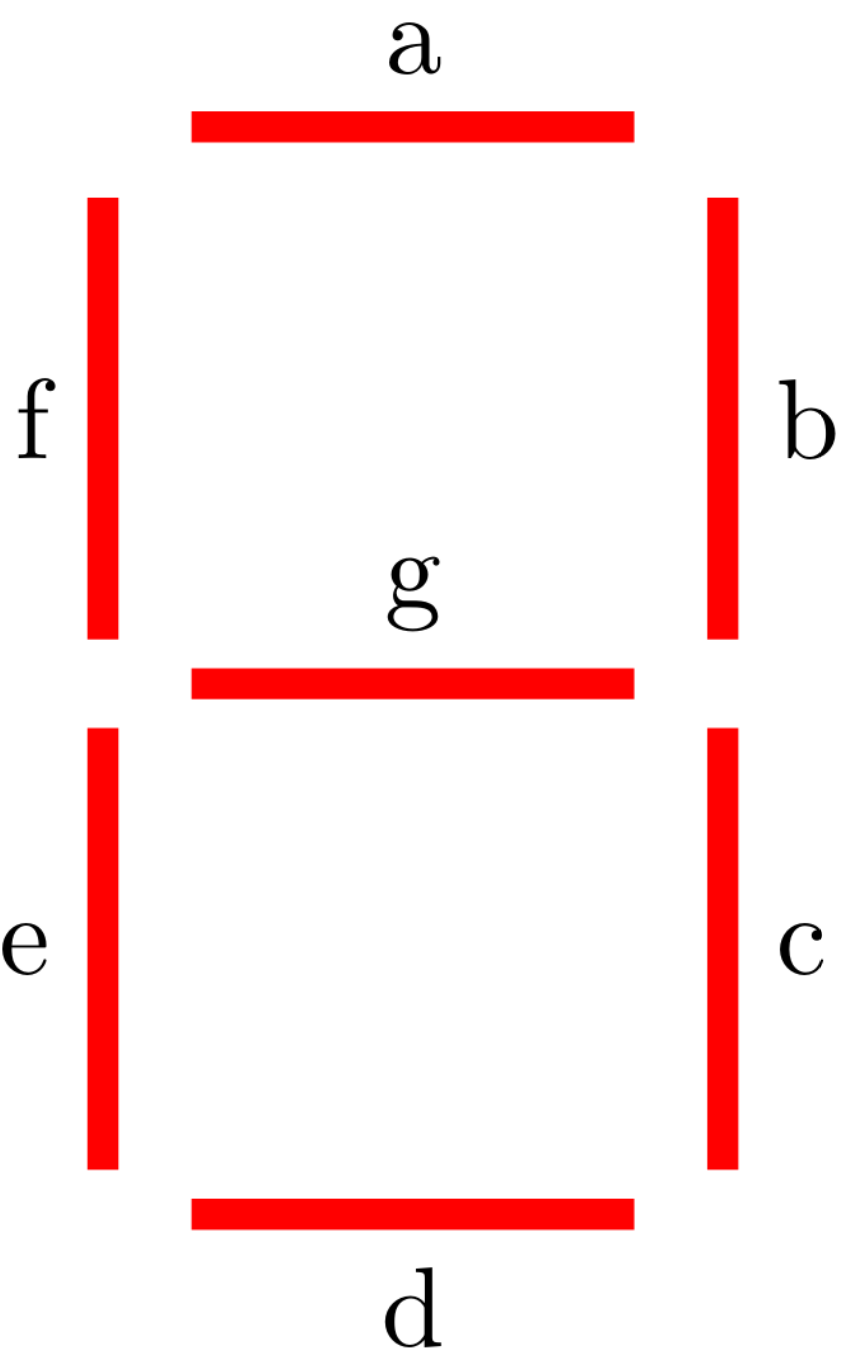
\includegraphics[width=0.85\linewidth]{./assets/abbildung-01-01.png}
    \vfill
\end{minipage}

\pagebreak

\section{Aufgabe 2}

Informieren Sie sich "uber die BCD Codierung. Schauen Sie in der gegebenen
Wertetabelle von Aufgabe 1 nach, bei welchen Eingangskonstellationen f"ur $x3$,
$x2$, $x1$, $x0$ das Segment $e$ leuchten soll. Stellen Sie mit den digitalen
Basis-Gattern eine Schaltung auf, deren Ausgang das Segment $e$ ansteuert.
(Ohne vorherige Optimierung, nur Gatter mit 1 oder 2 Eing"agen verwenden.)

Siehe circuits/circuit-02-01.circ

\section{Aufgabe 3}

Spielen Sie die Addition der beiden Zahlen $A = 10_10 = 1010_2$ und $B = 7_10 =
0111_2$ mit dem 4 Bit Paralleladdierer durch. Schreiben Sie dazu die Bits aus
der Rechnung jeweils an die Ein- und Ausg"ange des Addierers.

\vspace{5pt}

\begin{figure}[h]
    \centering
    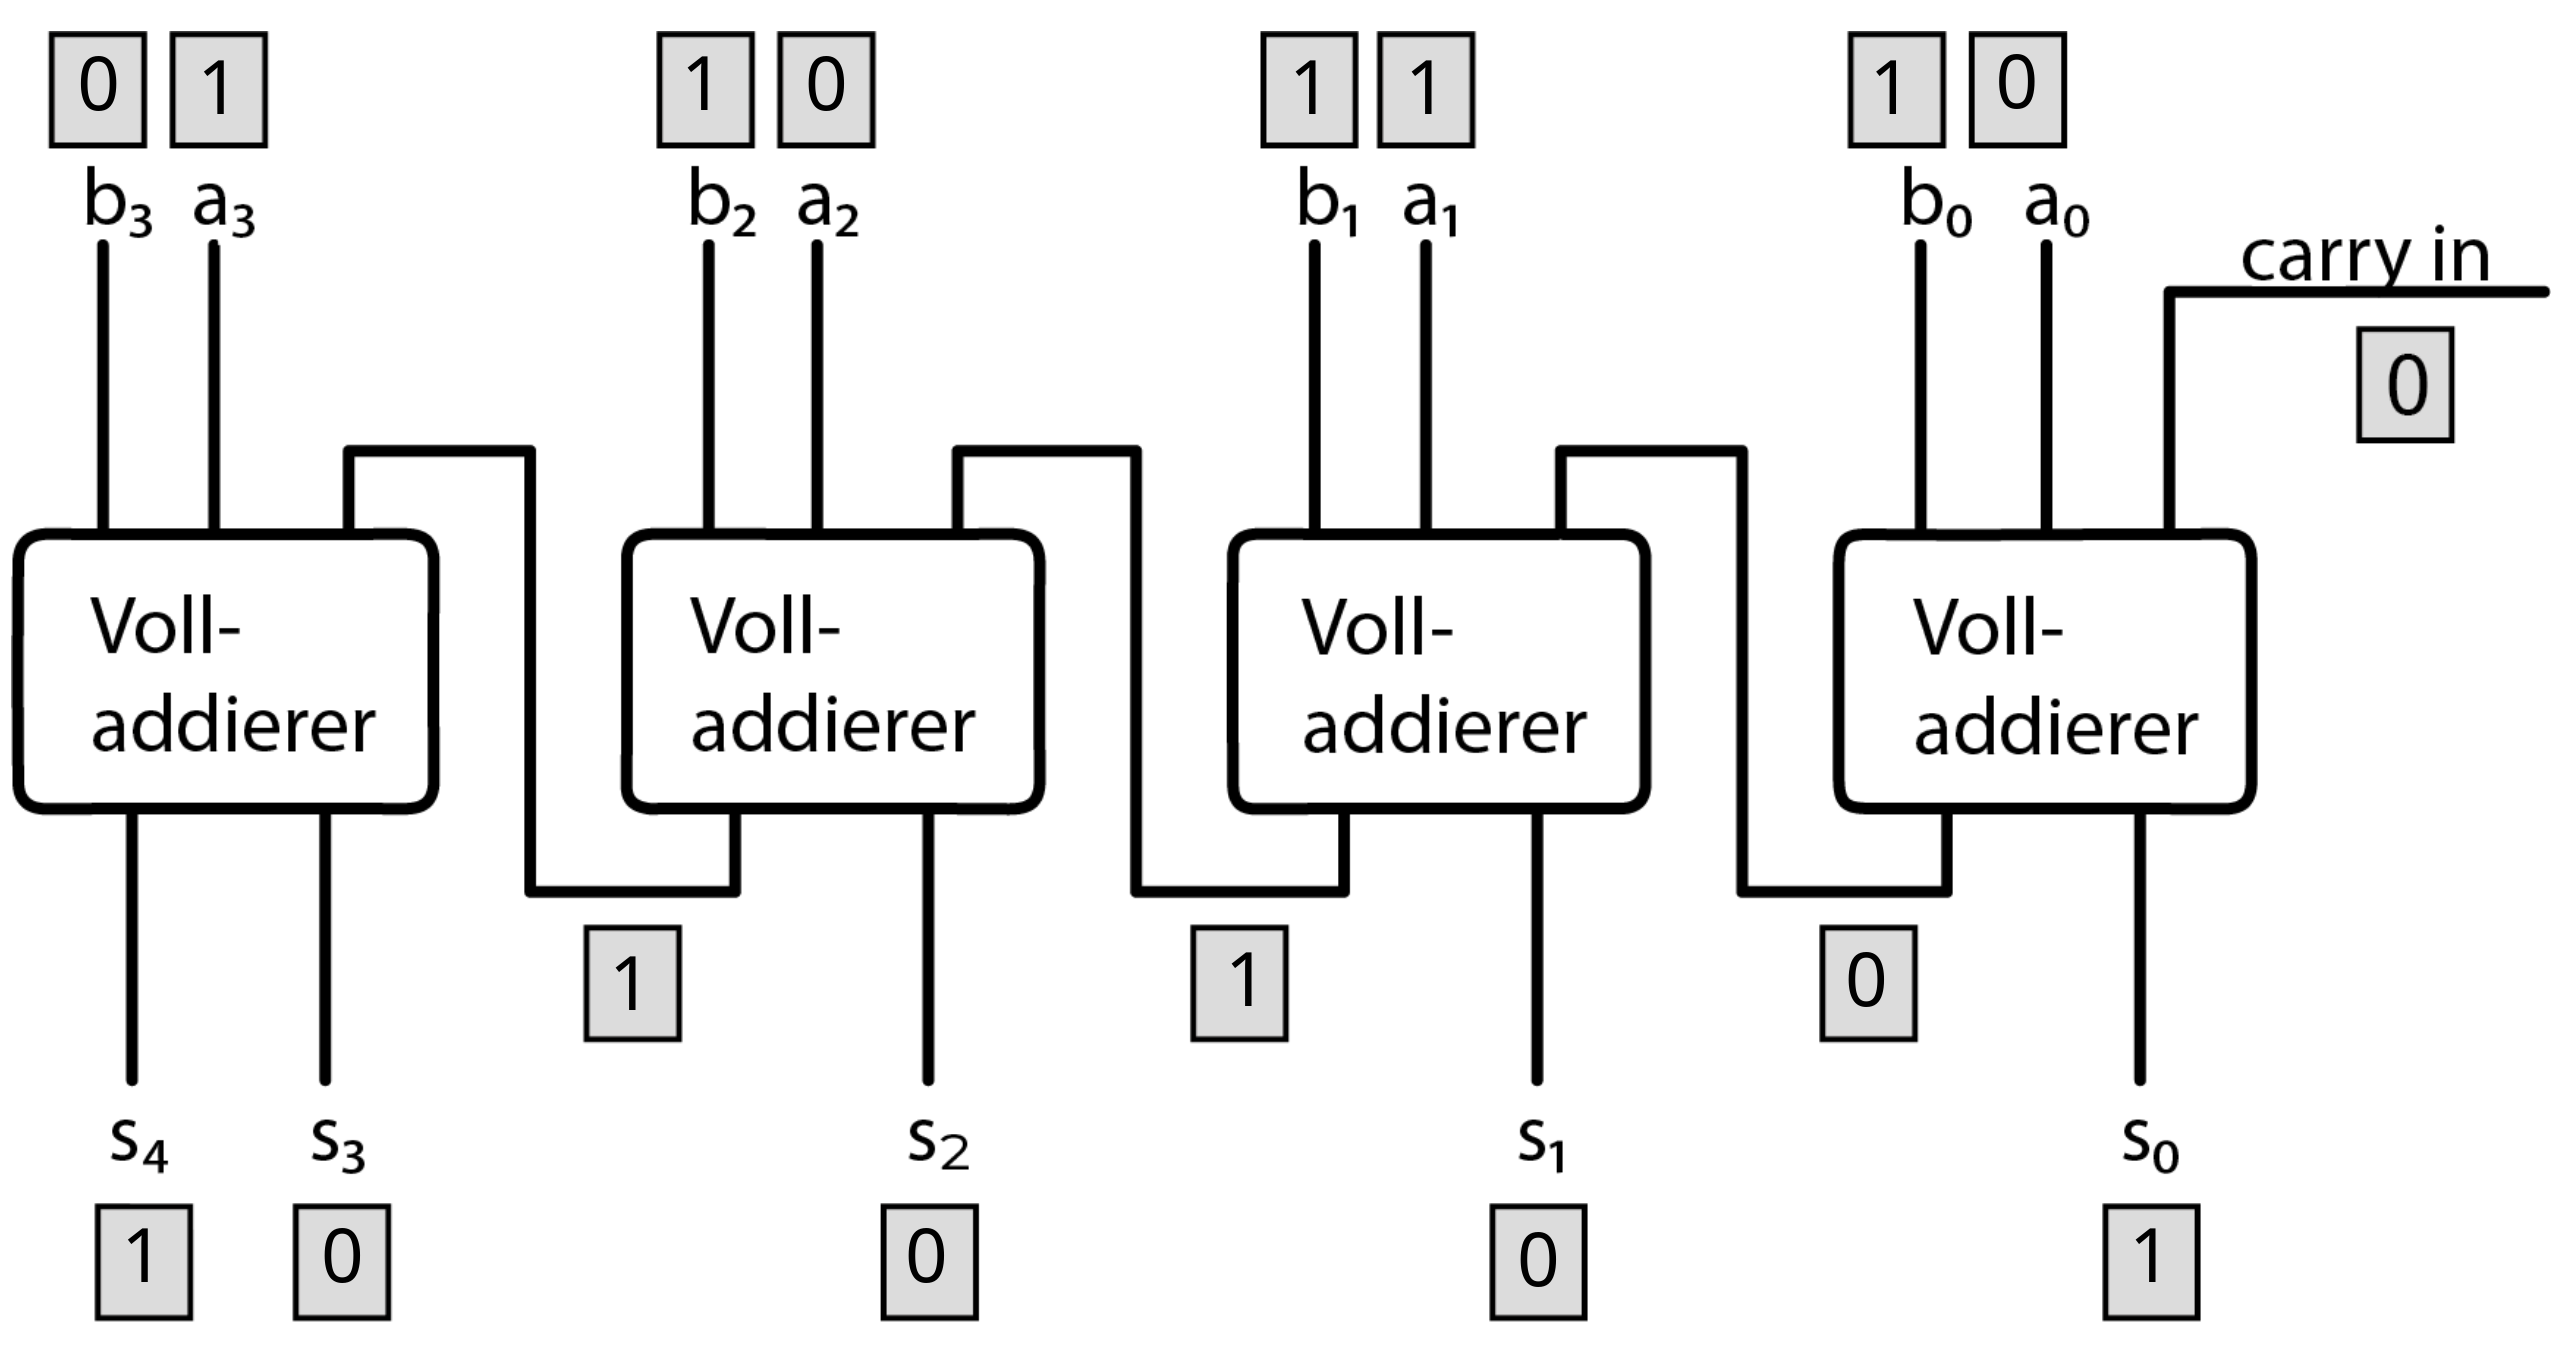
\includegraphics[width=0.8\textwidth]{./assets/abbildung-03-01.png}
    \caption{}
\end{figure}

\section{Aufgabe 4}

\begin{enumerate}[(a)]
    \item Wie viele Steuerleistungen ben"otigt ein Multiplexer f"ur 14 Eing"ange?
        \begin{equation*}
            n = {\lceil}{\log}_2(14){\rceil} = {\lceil}3.81{\rceil} = 4
        \end{equation*}

    \item Zeichnen Sie das logische Diagramm f"ur einen Multiplexer mit 1
        Steuerleitung und 2 Eing"angen. Verwenden Sie nur AND, OR und NOT
        Gatter. AND und OR Gatter d"urfen beliebig viele Eing"ange haben.
        Hinweis: Dann sollte ein NOT, zwei AND und ein OR ausreichen.

        Siehe circuits/circuit-04-01.circ
\end{enumerate}

\end{document}
